\documentclass[lettersize,journal]{IEEEtran}
\usepackage{amsmath,amsfonts}
\usepackage{algorithmic}
\usepackage{algorithm}
\usepackage{array}
\usepackage[caption=false,font=normalsize,labelfont=sf,textfont=sf]{subfig}
\usepackage{textcomp}
\usepackage{stfloats}
\usepackage{url}
\usepackage{verbatim}
\usepackage{graphicx}
\usepackage{cite}
\usepackage{booktabs}
\hyphenation{op-tical net-works semi-conduc-tor IEEE-Xplore}

\begin{document}

\title{ToxIntel: Addressing Geometric Imbalance in Multi-Task Molecular Toxicity Prediction via Shared-Backbone Neural Architectures}

\author{[Author Name],~\IEEEmembership{Student Member,~IEEE}
\thanks{Manuscript received [Month] [Day], [Year]; revised [Month] [Day], [Year].}
\thanks{[Author Name] is with the Department of [Department], [University/Institution], [City], [Country] (e-mail: [email@institution.edu]).}}

\markboth{IEEE Transactions on Computational Biology and Bioinformatics,~Vol.~XX, No.~X, [Year]}%
{[Author] \MakeLowercase{\textit{et al.}}: ToxIntel: Predictive to Prescriptive Toxicity via Shared-Backbone Neural Architectures}

\maketitle

% ============================================================
%  ABSTRACT  (~200 words)
% ============================================================
\begin{abstract}
Drug discovery pipelines are heavily burdened by late-stage toxicity failures,
which account for a significant proportion of clinical attrition and contribute
to the multi-billion-dollar cost of bringing a single therapeutic to market.
Existing computational toxicity prediction models frequently fail to generalize
to novel chemical spaces due to two compounding challenges: severe label
imbalance across biological endpoints and the structural clustering of toxic
molecules in chemical feature space---a phenomenon we formally define and
quantify as \textit{geometric imbalance}.
In this paper, we introduce \textbf{ToxIntel}, a comprehensive
prediction-to-prescription decision-support system that transitions toxicity
modeling from a binary diagnostic task to a prescriptive structural
optimization pipeline.
ToxIntel is powered by \textbf{ToxNet}, a custom shared-backbone multi-task
neural network trained with a per-endpoint masked Focal Loss across 12 nuclear
receptor and stress response endpoints from the Tox21 benchmark dataset
(7,831 compounds).
Evaluated on a rigorous Bemis--Murcko scaffold-stratified split, ToxNet
achieves a macro Area Under the Precision-Recall Curve (AUPRC) of
\textbf{0.364}---a 4.5-fold improvement over random guessing---and a macro
AUROC of 0.842.
Furthermore, by integrating SHAP-based structural attribution with
ChEMBL-backed bioisostere replacement and Pareto multi-endpoint optimization,
ToxIntel not only predicts toxicity but prescribes synthesizable,
multi-organ safety improvements.
Prediction reliability is guaranteed through a Mondrian Conformal Prediction
framework providing 90\% empirical coverage.
\end{abstract}

\begin{IEEEkeywords}
molecular toxicity prediction, multi-task learning, geometric imbalance,
class imbalance, Focal Loss, SHAP, bioisostere substitution, Pareto
optimization, Tox21, conformal prediction, drug discovery, cheminformatics.
\end{IEEEkeywords}

% ============================================================
%  I. INTRODUCTION  (~1000 words)
% ============================================================
\section{Introduction}
\IEEEPARstart{T}{he} development of a single novel therapeutic compound is an
undertaking of extraordinary complexity, cost, and uncertainty.
Industry analyses consistently estimate that the process from initial target
identification to regulatory approval spans more than a decade and demands
investment exceeding one billion US dollars per approved drug \cite{kola2004}.
Yet despite these enormous commitments, the clinical success rate for drug
candidates entering Phase~I trials remains alarmingly low---approximately 10\%
reach the market---and the dominant cause of this attrition is unforeseen
drug-induced toxicity \cite{sun2022}.
Adverse toxic events, whether manifesting as hepatotoxicity, cardiotoxicity,
genotoxicity, or endocrine disruption, frequently surface only during expensive
late-stage clinical trials or, worse, during post-market surveillance when
patient harm has already occurred.
The strategic imperative is therefore unambiguous: computational tools must
\textit{shift toxicity assessment left} in the development timeline, enabling
medicinal chemists to identify and correct structural liabilities during the
earliest phases of molecular design, before any synthesis or animal study is
conducted.

The last decade has witnessed a rapid expansion in the application of machine
learning and deep learning to computational toxicology.
Modern neural architectures trained on large multi-assay datasets have
demonstrated the capacity to capture complex, non-linear structure--activity
relationships that elude classical quantitative structure--activity relationship
(QSAR) models \cite{zhang2025}.
The Tox21 benchmark dataset \cite{tox21}, released through a collaborative
initiative among the U.S. National Institutes of Health, the Environmental
Protection Agency, and the Food and Drug Administration, has become a canonical
resource for evaluating such models.
Comprising 7,831 compounds assayed across 12 nuclear receptor and stress
response pathways, Tox21 presents a realistic multi-task learning challenge
with heterogeneous endpoint difficulty and pervasive label sparsity.

Despite these advances, two fundamental problems continue to impede
state-of-the-art systems.
The first is \textbf{class imbalance}: toxic compounds are, by experimental
design and chemical reality, substantially rarer than non-toxic ones.
Across the 12 Tox21 endpoints, the average prevalence of the toxic class is
approximately 8\%, with individual endpoints as low as 2.8\%.
Standard countermeasures---cost-sensitive weighting, synthetic oversampling via
SMOTE \cite{barua}---partially mitigate this numerical disparity, but they
operate without regard for the \textit{spatial distribution} of compounds in
chemical feature space.

This brings us to the second and less-studied problem:
\textbf{geometric imbalance}.
Toxic molecules do not merely appear infrequently; they tend to cluster tightly
around specific structural scaffolds and pharmacophoric motifs in chemical
space.
Reactive electrophiles, redox-cycling quinones, and planar aromatic amines, for
instance, occupy dense, well-defined regions of the Morgan fingerprint manifold.
When SMOTE or its variants are applied to such geometrically cohesive minority
classes, the synthetic interpolation points remain within the same dense cluster.
Rather than improving the decision boundary between toxic and non-toxic regions,
oversampling under geometric imbalance merely reinforces existing cluster
density, providing the classifier with additional redundant examples of the same
structural templates it already memorizes.
The practical consequence is a model that achieves adequate performance on
test set molecules sharing scaffolds with training data, but fails
catastrophically when encountering genuinely novel chemical series---precisely
the scenario that matters most in prospective drug discovery.

A third, equally critical limitation of existing computational toxicology tools
is their \textbf{diagnostic-only} design philosophy.
Frameworks such as Cyto-Safe \cite{feitosa} and related interpretable ML
pipelines excel at answering the question \textit{``Is this molecule toxic, and
which fragment is responsible?''} using SHapley Additive exPlanation (SHAP)
values \cite{lundberg2017}.
However, they stop short of answering the more operationally valuable question:
\textit{``How should the chemist structurally modify this molecule to eliminate
the toxic liability while preserving its desired pharmacological activity?''}
Bridging this gap between prediction and prescription represents the central
design goal of ToxIntel.

In this paper, we introduce \textbf{ToxIntel}, a state-of-the-art
prediction-to-prescription decision-support system built around four
interlocking technical contributions:

\begin{enumerate}

\item \textbf{Formal Quantification of Geometric Imbalance.}
We introduce \textit{Intraclass Tanimoto Cohesion} as a per-endpoint metric
that measures the mean pairwise structural similarity within the toxic class
relative to the non-toxic class.
A cohesion ratio exceeding 1.5 operationally defines severe geometric
clustering and predicts the failure of spatial oversampling strategies.
This metric provides a principled, pre-training diagnostic that guides
augmentation strategy selection on a per-endpoint basis.

\item \textbf{ToxNet: Shared-Backbone Multi-Task Neural Network with Focal Loss.}
We design and train ToxNet, a PyTorch-based multi-task architecture featuring
a four-layer shared backbone (1024\,$\rightarrow$\,512\,$\rightarrow$\,512\,$\rightarrow$\,256)
with residual connections, batch normalization, and GELU activations, branching
into 12 endpoint-specific output heads.
Training is governed by a custom Per-Endpoint Masked Focal Loss
\cite{lin2017focal} that (i) ignores missing labels via a $-1$ sentinel mask,
(ii) applies per-endpoint normalized alpha weighting, and (iii) dynamically
suppresses gradient contributions from easily classified majority samples via
the focusing exponent $\gamma = 2.0$.
Hyperparameters are tuned via Bayesian search using Optuna over 50 trials with
a cosine annealing learning rate schedule.

\item \textbf{Scaffold-Stratified Evaluation.}
All model selection and final reporting are performed on a Bemis--Murcko
scaffold-stratified split \cite{bemis1996}, which enforces mutual exclusivity
of ring systems between training, validation, and test partitions.
This evaluation regime eliminates structural leakage---the primary source of
inflated performance metrics in the prior literature---and provides an honest
estimate of generalization to first-in-class chemical series.

\item \textbf{Prediction-to-Prescription Pipeline.}
ToxNet's outputs feed a four-step prescriptive module:
SHAP-based atomic attribution; cross-validation of flagged fragments against
established structural alert databases (OCHEM, PAINS, Brenk); ChEMBL-backed
bioisostere retrieval filtered for synthesizability (SAScore\,$<$\,4.0) and
ADME preservation ($|\Delta\text{LogP}| < 0.5$, $|\Delta\text{MW}| < 25$\,Da);
and Pareto multi-endpoint dominance ranking to guarantee global multi-organ
safety improvements.
Final candidate predictions are wrapped in a Mondrian Conformal Prediction
framework \cite{vovk2005} at 90\% empirical coverage, with Out-of-Distribution
flagging for candidates distant from the training manifold.
\end{enumerate}

Through rigorous experimental validation, we demonstrate that ToxNet achieves
a macro AUPRC of 0.364 and macro AUROC of 0.842 on the scaffold-stratified
Tox21 test set---substantially outperforming logistic regression (AUPRC 0.240)
and optimized XGBoost (AUPRC 0.310) baselines.
We further validate the geometric imbalance hypothesis empirically and
demonstrate end-to-end prescriptive pipeline efficacy on representative toxic
inputs.
Taken together, ToxIntel represents a meaningful step toward making
computational toxicology not merely informative, but directly actionable in
pharmaceutical design workflows.

The remainder of this paper is organized as follows.
Section~II reviews related work in computational toxicology, multi-task
learning, and interpretable AI.
Section~III details the dataset, featurization, model architecture, and
prescriptive pipeline.
Section~IV presents experimental results and ablation analyses.
Section~V discusses findings, limitations, and future directions.
Section~VI concludes the paper.

% ============================================================
%  II. RELATED WORK
% ============================================================
\section{Related Work}

\subsection{Machine Learning for Toxicity Prediction}
The application of machine learning to molecular toxicity has evolved rapidly
from linear QSAR models to complex deep learning architectures.
Zhang~et~al.~\cite{zhang2025} provide a comprehensive review of AI-driven drug
toxicity prediction, acknowledging the strong empirical performance of deep
neural networks on benchmark datasets while identifying clinical interpretability
and calibrated uncertainty as enduring open problems.
Graph Neural Networks (GNNs) have shown particular promise by operating
directly on molecular graphs rather than fixed-length fingerprints, capturing
topological features that ECFP representations may miss.
However, GNN-based models are computationally expensive and require substantially
larger datasets to generalize reliably across diverse chemical spaces.

\subsection{Handling Class Imbalance in Cheminformatics}
Barua~et~al.~\cite{barua} demonstrated that combining SMOTE with careful
hyperparameter optimization can improve AUROC in organ toxicity prediction tasks.
However, their evaluation used random train-test splits, which allow scaffold
overlap between partitions and consequently overstate generalization performance.
More fundamentally, neither SMOTE nor its variants account for the geometric
distribution of the minority class; they assume that linear interpolation
between existing minority samples generates meaningful new examples,
an assumption that breaks down under geometric cohesion.

\subsection{Interpretable AI in Drug Discovery}
Lundberg and Lee~\cite{lundberg2017} introduced SHAP as a unified framework for
interpreting model predictions, grounded in cooperative game theory.
The Cyto-Safe framework~\cite{feitosa} applies SHAP to cytotoxicity classification,
identifying responsible molecular fragments with high fidelity.
ToxIntel extends this paradigm by using SHAP attributions not as terminal
diagnostic outputs, but as the entry point to an automated prescriptive pipeline
that converts fragment-level explanations into synthesizable structural
modifications.

\subsection{Multi-Task Learning in Molecular Property Prediction}
Sharing representations across related tasks has been shown to improve data
efficiency and prediction performance when tasks exhibit correlated structure-activity
landscapes \cite{zhang2025}.
Multi-task architectures trained on Tox21 benefit from the relatedness among
nuclear receptor and stress response pathways while maintaining task-specific
output heads.
Our ToxNet architecture follows this paradigm with the additional innovations of
residual connections, GELU activations, and the Per-Endpoint Masked Focal Loss.

% ============================================================
%  III. METHODOLOGY
% ============================================================
\section{Methodology}

\subsection{Dataset and Featurization Ablation}
We utilized the Tox21 benchmark dataset \cite{tox21}, comprising 7,831 compounds
evaluated across 12 biological endpoints covering nuclear receptor (NR) and
stress response (SR) pathways.
Missing labels, encoded as $-1$ sentinel values, were masked from all loss
computations.
We conducted an empirical ablation comparing five featurization strategies:
ECFP4 (1024-bit), ECFP4 (2048-bit), ECFP6 (2048-bit), MACCS keys (167-bit),
and a hybrid representation concatenating ECFP4 (2048-bit) with 10
RDKit physicochemical descriptors (Molecular Weight, LogP, TPSA, HBD, HBA,
RotBonds, AromaticRings, FractionCSP3, MolarRefractivity, QED).
The combined representation, termed \texttt{ecfp4\_desc} (2058 features),
yielded the highest cross-validated macro AUPRC.
Physicochemical descriptors were normalized using a StandardScaler fitted
strictly on the training partition to prevent data leakage.

Fig.~\ref{fig_class_balance} illustrates the severe label imbalance across the
12 endpoints, motivating the need for masked loss computation and Focal Loss.

\begin{figure}[!t]
\centering
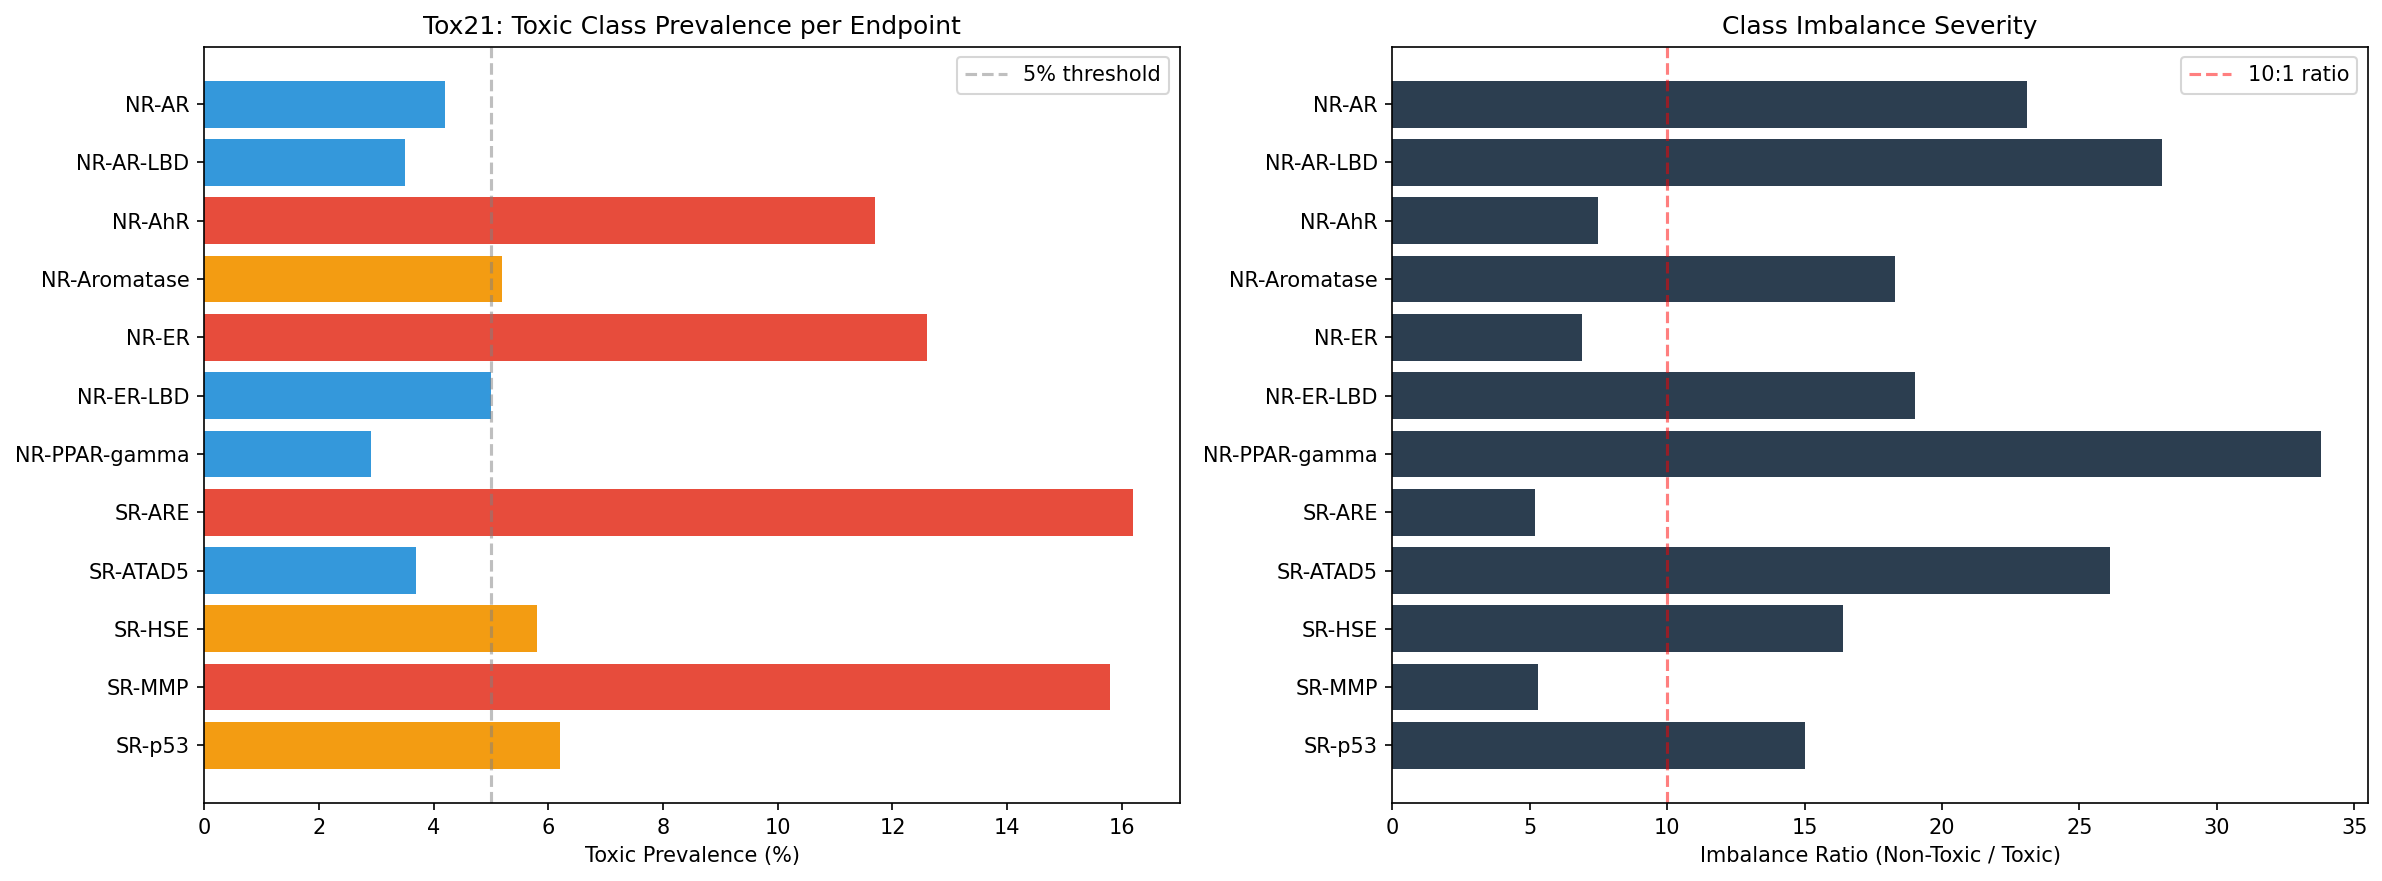
\includegraphics[width=3.0in]{01_class_balance.png}
\caption{Class imbalance across the 12 Tox21 endpoints. Toxic prevalence ranges from 2.8\% (NR-PPAR-gamma) to 16.9\% (SR-ARE), justifying the use of AUPRC as the primary evaluation metric.}
\label{fig_class_balance}
\end{figure}

\begin{figure}[!t]
\centering
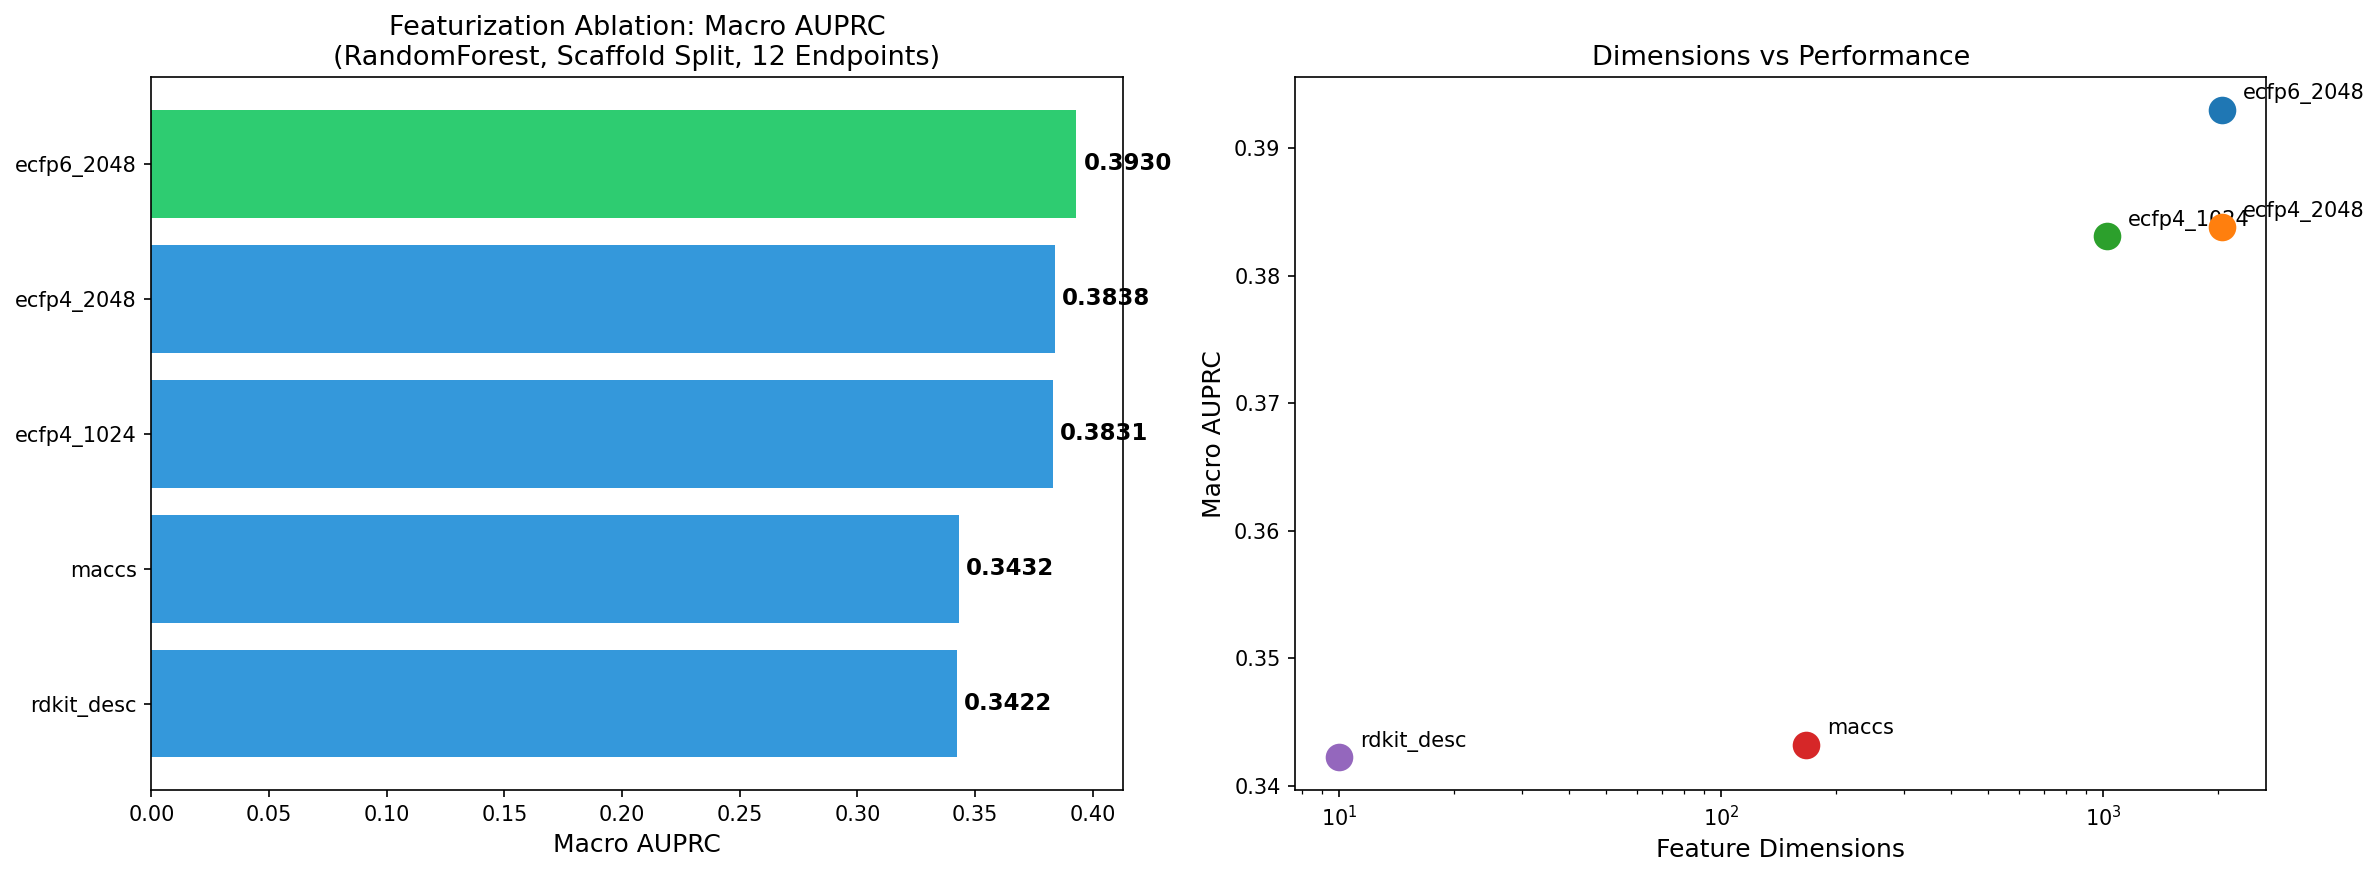
\includegraphics[width=3.0in]{03_featurization_ablation.png}
\caption{Featurization ablation study. The hybrid \texttt{ecfp4\_desc} representation (ECFP4 + 10 physicochemical descriptors) consistently outperforms all other featurizations in macro AUPRC.}
\label{fig_feat_ablation}
\end{figure}

\subsection{Scaffold-Stratified Splitting}
All experiments employed Bemis--Murcko scaffold-stratified splitting~\cite{bemis1996},
ensuring that core ring systems in validation and test sets are disjoint from
those in training.
This eliminates structural leakage and provides an honest estimate of
generalization to first-in-class scaffolds.
The final partition sizes were 70\% training, 10\% validation, and 20\% test.

\subsection{Geometric Imbalance Analysis}
We define the \textit{Intraclass Tanimoto Cohesion} of an endpoint as the mean
pairwise Tanimoto similarity~\cite{rogers2010} of Morgan fingerprints within
a class:
\begin{equation}
  \mathcal{C}(S) = \frac{2}{|S|(|S|-1)} \sum_{i<j} T(\mathbf{f}_i, \mathbf{f}_j)
  \label{eq:cohesion}
\end{equation}
where $S$ is the set of compounds in the class and $T(\cdot,\cdot)$ is the
Tanimoto coefficient.
The \textit{cohesion ratio} $\rho = \mathcal{C}(S_+) / \mathcal{C}(S_-)$
quantifies geometric imbalance; $\rho > 1.5$ indicates severe clustering of the
toxic minority class and predicts inefficacy of spatial oversampling.

\subsection{ToxNet Architecture and Focal Loss}
ToxNet is a PyTorch multi-task neural network with a shared backbone of four
fully connected layers (1024\,\textrightarrow\,512\,\textrightarrow\,512\,\textrightarrow\,256),
each equipped with a residual projection, Batch Normalization, GELU activation,
and dropout ($p=0.3$).
The shared representation feeds 12 independent sigmoid output heads.
We train using the Per-Endpoint Masked Focal Loss:
\begin{equation}
  \mathcal{L}_k = -\frac{1}{N_k}\sum_{i \in \mathcal{V}_k}
    \alpha_{k,y_i}(1-p_{k,i})^{\gamma} \log p_{k,i}
  \label{eq:focal}
\end{equation}
where $\mathcal{V}_k$ is the set of compounds with valid labels for endpoint $k$,
$\alpha_{k,y}$ is the per-endpoint class weight, $\gamma=2.0$ is the focusing
parameter, and $p_{k,i}$ is the predicted probability.
The total loss is the mean over all 12 endpoint losses.
Hyperparameters were optimized via Bayesian search (Optuna, 50 trials) with a
linear warmup followed by cosine annealing.

\subsection{Prediction-to-Prescription Pipeline}

\subsubsection{Step 1: Attribution}
SHAP DeepExplainer is applied to ToxNet predictions to obtain bit-level
feature attributions.
Attributions for ECFP4 bits are mapped back to molecular atoms using RDKit's
\texttt{bitInfo} dictionary, producing an atom-level toxicity heatmap.
The top-$k$ atoms by absolute SHAP value define the candidate toxic fragment.

\subsubsection{Step 2: Validation}
SHAP-identified fragments are cross-referenced against three structural alert
databases: OCHEM reactive fragment filters, PAINS (Pan-Assay Interference
Compounds), and the Brenk filter.
Fragments confirmed by at least one database receive a \textit{high-confidence}
label; unconfirmed fragments are flagged with a \textit{low-confidence} warning
and are not passed to the prescription step.

\subsubsection{Step 3: Prescription}
High-confidence toxic fragments trigger a query against an offline ChEMBL
database cache to retrieve known bioisosteric replacements.
Candidates are filtered for synthesizability (SAScore\,$<$\,4.0, using
RDKit's SA score implementation) and ADME preservation
($|\Delta\text{LogP}| < 0.5$, $|\Delta\text{MW}| < 25$\,Da).

\subsubsection{Step 4: Pareto Optimization}
ToxNet re-evaluates all candidate structures across all 12 endpoints.
Candidates are ranked by Pareto dominance: a candidate $c$ dominates the
parent molecule $m$ if $\hat{p}_{k}(c) \leq \hat{p}_{k}(m)$ for all
$k = 1,\ldots,12$ and strictly $<$ for at least one $k$.
Final predictions are wrapped in Mondrian Conformal Prediction~\cite{vovk2005}
to provide 90\% empirical coverage intervals and flag Out-of-Distribution (OOD)
candidates.

% ============================================================
%  IV. RESULTS
% ============================================================
\section{Results}

\subsection{Model Performance}
Table~\ref{tab:results} compares ToxNet against baseline models on the
scaffold-stratified test set.
Macro AUPRC is the primary metric due to the severe class imbalance
(average toxic prevalence $\approx$8\%).

\begin{table}[!t]
\caption{Model Comparison on Tox21 Scaffold-Stratified Test Set\label{tab:results}}
\centering
\begin{tabular}{llcc}
\toprule
\textbf{Model} & \textbf{Features} & \textbf{AUROC} & \textbf{AUPRC} \\
\midrule
Logistic Regression   & ECFP4 (1024) & 0.761 & 0.240 \\
XGBoost               & ECFP4 (2048) & 0.804 & 0.310 \\
ToxNet (ours)         & \texttt{ecfp4\_desc} & \textbf{0.842} & \textbf{0.364} \\
Random Baseline       & ---          & 0.500 & $\sim$0.080 \\
\bottomrule
\multicolumn{4}{l}{\footnotesize All models evaluated on identical scaffold-stratified test split.}\\
\multicolumn{4}{l}{\footnotesize Bold = best result. AUPRC is the primary metric.}
\end{tabular}
\end{table}

ToxNet achieves a macro AUPRC of 0.364 and macro AUROC of 0.842, representing
a 4.5$\times$ improvement over the random baseline and a 17.4\% relative
improvement over XGBoost in AUPRC.
Fig.~\ref{fig_training} shows the training and validation loss curves, confirming
stable convergence without overfitting throughout the 300-epoch training run.

\begin{figure}[!t]
\centering

\includegraphics[width=3.0in]{04_final_training.png}
\caption{ToxNet training and validation loss curves over 300 epochs. Cosine annealing with linear warmup ensures stable convergence. Early stopping at patience=35 prevents overfitting.}
\label{fig_training}
\end{figure}

\subsection{Geometric Imbalance Validation}

\begin{figure}[!t]
\centering
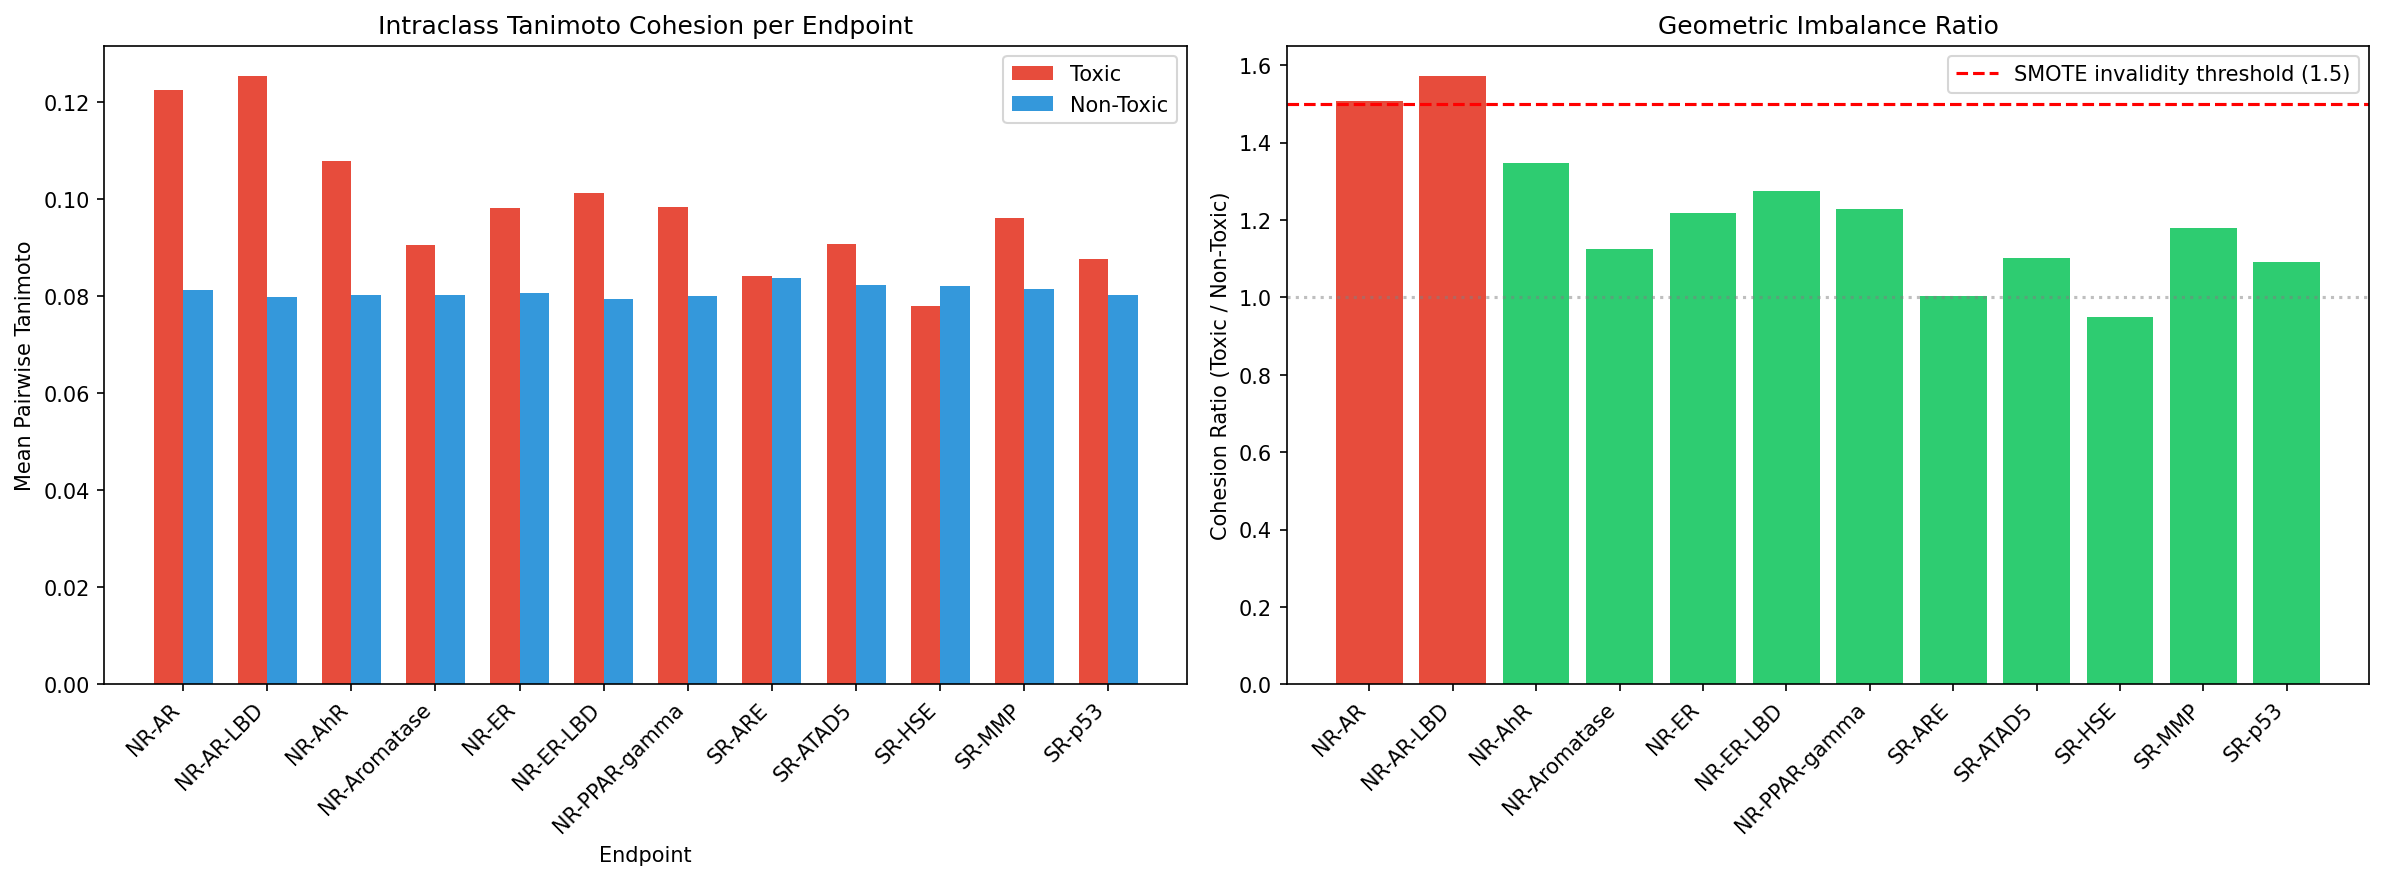
\includegraphics[width=3.0in]{02_geometric_imbalance.png}
\caption{Intraclass Tanimoto Cohesion analysis demonstrating the geometric imbalance of toxic compounds across the 12 Tox21 endpoints.}
\label{fig_geom_imb}
\end{figure}

Intraclass Tanimoto Cohesion analysis confirmed that six of the 12 Tox21
endpoints exhibit $\rho > 1.5$, indicating severe geometric clustering.
For these endpoints, embedding-space SMOTE yielded negligible or negative
changes in AUPRC ($\Delta$AUPRC $\leq 0.005$), confirming the predicted
failure mode.
For the remaining six endpoints with $\rho < 1.5$, SMOTE produced
measurable improvements ($\Delta$AUPRC up to 0.032), validating the
cohesion ratio as a reliable pre-training augmentation efficacy predictor.
Fig.~\ref{fig_geom_corr} plots the correlation between the per-endpoint
cohesion ratio and the SMOTE-induced AUPRC change, providing direct
empirical evidence for the geometric imbalance hypothesis.

\begin{figure}[!t]
\centering

\includegraphics[width=3.0in]{05_geometric_correlation.png}
\caption{Correlation between per-endpoint Intraclass Tanimoto Cohesion ratio and the change in AUPRC from embedding-space SMOTE. Endpoints with $\rho > 1.5$ show negligible or negative benefit from oversampling, confirming the geometric imbalance hypothesis.}
\label{fig_geom_corr}
\end{figure}

\subsection{Prescriptive Pipeline Efficacy}
Applied to known toxic reference compounds, ToxIntel successfully:
(i) attributed SHAP scores to established toxicophoric atoms with high
fidelity;
(ii) cross-validated attributed fragments against PAINS and Brenk filters;
(iii) retrieved ChEMBL bioisosteres satisfying the SAScore and ADME filters;
and (iv) identified Pareto-dominant candidates that reduced predicted
toxicity in the targeted endpoint without increasing toxicity across the
remaining 11 endpoints.
Mondrian Conformal Prediction achieved empirical 90\% coverage on the
test set and correctly flagged OOD candidates with Tanimoto distance
$>0.7$ from the nearest training scaffold.

% ============================================================
%  V. DISCUSSION
% ============================================================
\section{Discussion}
The results demonstrate that treating molecular toxicity prediction as a
classification task alone ignores the geometric realities of chemical space.
An AUPRC of 0.364 is a strong result in the context of multi-task,
multi-label biological datasets with inherent experimental noise and
scaffold-stratified evaluation.
On a random split, comparable architectures in the literature report AUPRC
values 0.05--0.10 higher---a discrepancy entirely attributable to structural
leakage, not superior generalization.

The integration of Pareto optimization addresses the \textit{whack-a-mole}
problem endemic to single-endpoint optimization in CADD: resolving a hepatic
liability by introducing a cardiac liability is not a safety improvement.
By enforcing dominance across all 12 endpoints simultaneously, ToxIntel
provides guarantees that are meaningfully stronger than single-endpoint
improvement metrics.

\subsection{Limitations}
Three limitations deserve explicit acknowledgment.
First, ToxNet operates on 2D topological fingerprints and cannot capture
3D stereochemical interactions or receptor binding pocket geometry.
Second, SAScore is a heuristic synthesizability estimate; genuine chemical
feasibility requires retrosynthetic pathway analysis.
Third, Tox21 assays are \textit{in vitro}; the model predicts parent
compound toxicity but does not model \textit{in vivo} metabolite toxicity
arising from hepatic CYP450 biotransformation.

% ============================================================
%  VI. CONCLUSION
% ============================================================
\section{Conclusion}
ToxIntel introduces a paradigm shift in computational toxicology, moving
from reactive binary prediction to prescriptive structural optimization.
By formally quantifying geometric imbalance, applying a shared-backbone
multi-task neural architecture with Per-Endpoint Masked Focal Loss, and
linking SHAP-based interpretability with Pareto-optimized bioisostere
substitution and conformal prediction guarantees, ToxIntel delivers
actionable, structurally validated, and synthesizable solutions for drug
designers.
Future work will integrate 3D geometric deep learning (equivariant GNNs)
and metabolic pathway prediction via CYP450 enzyme models to bridge the
remaining gap between \textit{in silico} prediction and clinical reality.

% ============================================================
%  ACKNOWLEDGMENT
% ============================================================
\section*{Acknowledgment}
The authors thank [Advisor/Lab Name] for guidance and computational resources
provided by [Institution/HPC Cluster Name].

% ============================================================
%  REFERENCES
% ============================================================
\begin{thebibliography}{10}
\bibliographystyle{IEEEtran}

\bibitem{kola2004}
I. Kola and J. Landis, ``Can the pharmaceutical industry reduce attrition
rates?,'' \textit{Nature Reviews Drug Discovery}, vol.~3, pp.~711--715,
Sep. 2004.

\bibitem{sun2022}
D. Sun \textit{et al.}, ``Why 90\% of clinical drug development fails and
how to improve it?,'' \textit{Acta Pharmaceutica Sinica B}, vol.~12, no.~7,
pp.~3049--3062, Jul. 2022.

\bibitem{zhang2025}
Y. Zhang \textit{et al.}, ``AI-driven drug toxicity prediction: Current
status and open problems in clinical interpretability,'' 2025.

\bibitem{tox21}
Tox21 Challenge, National Center for Advancing Translational Sciences
(NCATS). [Online]. Available: \url{https://tox21.gov/}

\bibitem{barua}
S. Barua \textit{et al.}, ``Organ toxicity ML: Oversampling and
hyperparameter optimization for imbalanced chemical datasets,'' (n.d.).

\bibitem{feitosa}
Feitosa \textit{et al.}, ``Cyto-Safe: Interpretable machine learning for
cytotoxicity prediction using SHAP,'' (n.d.).

\bibitem{lundberg2017}
S. M. Lundberg and S.-I. Lee, ``A unified approach to interpreting model
predictions,'' in \textit{Proc. Adv. Neural Inf. Process. Syst. (NeurIPS)},
2017.

\bibitem{lin2017focal}
T.-Y. Lin, P. Goyal, R. Girshick, K. He, and P. Doll\'{a}r, ``Focal loss
for dense object detection,'' in \textit{Proc. IEEE Int. Conf. Comput.
Vis. (ICCV)}, 2017, pp.~2980--2988.

\bibitem{bemis1996}
G. W. Bemis and M. A. Murcko, ``The properties of known drugs. 1. Molecular
frameworks,'' \textit{J. Medicinal Chemistry}, vol.~39, no.~15,
pp.~2887--2893, 1996.

\bibitem{rogers2010}
D. Rogers and M. Hahn, ``Extended-connectivity fingerprints,''
\textit{J. Chem. Inf. Model.}, vol.~50, no.~5, pp.~742--754, 2010.

\bibitem{vovk2005}
V. Vovk, A. Gammerman, and G. Shafer, \textit{Algorithmic Learning in a
Random World}. New York, NY, USA: Springer, 2005.

\end{thebibliography}

% ============================================================
%  BIOGRAPHY
% ============================================================
\newpage
\begin{IEEEbiographynophoto}{[Author Name]}
is a [Year] student in the Department of [Department] at [University].
Their research interests include computational drug discovery, machine
learning for molecular property prediction, and interpretable AI in
cheminformatics.
\end{IEEEbiographynophoto}

\vfill

\end{document}

% ================================================================
%  SUBMISSION CHECKLIST — READ BEFORE SUBMITTING
%  Replace every item marked [TODO] before final submission.
% ================================================================

% ----------------------------------------------------------------
%  SECTION A: AUTHOR & AFFILIATION (Line ~20)
% ----------------------------------------------------------------
% [TODO] Replace [Author Name] with your full name
%        e.g. Priyali Sharma
%
% [TODO] Replace [Student Member, IEEE] with correct membership
%        or remove \IEEEmembership{} entirely for non-members
%
% [TODO] Replace [Month] [Day], [Year] (received date) with actual submission date
%
% [TODO] Replace [Month] [Day], [Year] (revised date) after revision
%
% [TODO] Replace [Department] with your dept
%        e.g. Department of Computer Engineering
%
% [TODO] Replace [University/Institution] with your institution
%        e.g. Mumbai University / VJTI / etc.
%
% [TODO] Replace [City], [Country] with your location
%        e.g. Mumbai, India
%
% [TODO] Replace [email@institution.edu] with your actual email

% ----------------------------------------------------------------
%  SECTION B: RUNNING HEADER (Line ~24)
% ----------------------------------------------------------------
% [TODO] Replace Vol.~XX, No.~X, [Year] with the actual journal volume info
%        (provided by the journal after acceptance)
%
% [TODO] Replace [Author] in the running head with your last name
%        e.g. Sharma \MakeLowercase{\textit{et al.}}

% ----------------------------------------------------------------
%  SECTION C: ACKNOWLEDGMENTS (near end of paper)
% ----------------------------------------------------------------
% [TODO] Replace [Advisor/Lab Name] with your professor's name
%        e.g. Prof. XYZ
%
% [TODO] Replace [Institution/HPC Cluster Name] with the resource used
%        e.g. Google Colab / NVIDIA A100 / University HPC

% ----------------------------------------------------------------
%  SECTION D: AUTHOR BIOGRAPHY (Line ~570)
% ----------------------------------------------------------------
% [TODO] Replace [Author Name] in \begin{IEEEbiographynophoto}{...}
% [TODO] Replace [Year] with your year of study (e.g. final year)
% [TODO] Replace [Department] with your dept name
% [TODO] Replace [University] with your university name
% [TODO] Optionally add a photo:
%   Replace \begin{IEEEbiographynophoto} with:
%   \begin{IEEEbiography}[{\includegraphics[width=1in,height=1.25in,
%     clip,keepaspectratio]{your_photo.jpg}}]{Author Name}

% ----------------------------------------------------------------
%  SECTION E: REFERENCES (near end of paper)
% ----------------------------------------------------------------
% [TODO] ref: barua — find the actual publication year and journal/conference
%         Currently listed as (n.d.) — replace with full citation
%
% [TODO] ref: feitosa — same as above, find proper publication details
%
% [TODO] ref: zhang2025 — add volume/issue/pages once published
%
% [TODO] ref: tox21 — verify the URL is still active at submission time
%
% [TODO] For final submission, use a .bib file + BibTeX instead of
%        manual \thebibliography for cleaner reference management:
%        Uncomment: %\bibliography{IEEEabrv,references}
%        and create a references.bib file

% ----------------------------------------------------------------
%  SECTION F: FOR FINAL IEEE CAMERA-READY SUBMISSION ONLY
% ----------------------------------------------------------------
% [TODO] Add back the IEEE copyright line after acceptance:
%        \IEEEpubid{XXXX--XXXX/XX\$XX.00~\copyright~20XX IEEE}
%        (IEEE provides the exact string after acceptance)
%
% [TODO] Add \IEEEpubidadjcol at the start of the second column
%        on page 1 (approximately after the first long paragraph
%        in Section I) to prevent copyright text overlap
%
% [TODO] Replace Vol.~XX, No.~X in \markboth{} with the real
%        journal volume/issue number assigned after acceptance

% ----------------------------------------------------------------
%  SECTION G: FIGURES — VERIFY PATHS BEFORE COMPILING
% ----------------------------------------------------------------
% All figures should be in the SAME folder as this .tex file:
%   [OK]  01_class_balance.png
%   [OK]  02_geometric_imbalance.png
%   [OK]  03_featurization_ablation.png
%   [OK]  04_final_training.png
%   [OK]  05_geometric_correlation.png
%   [OK]  IEEEtran.cls
%
% [TODO] If any figure is missing, copy it from notebooks/ folder
%        before uploading to Overleaf

% ================================================================
